\chapter{Introduction}
\label{ch:intro}
Computer systems have become an integral part of our daily life and are being used in various environments (such as homes, hospitals, factories) and application areas (such as medical devices, aircraft flight control, weapons, and nuclear systems) where failure could lead to loss of life, financial loss, or environmental damage. It is vital to verify the soundness and safety of such critical applications. Formal verification is increasingly applied to critical systems to ensure they work in all cases. It is the process of mathematically proving or disproving the correctness of a system with respect to certain requirements or properties.

One of the most successful and powerful methods for formal verification is symbolic model checking. Symbolic model checking using induction-based techniques such as IC3/PDR~\cite{Een2011:PDR} and $k$-induction~\cite{SheeranSS00} can often determine whether safety properties hold of complex finite or infinite-state systems.  Model checking tools are attractive both because they are automated, requiring little or no interaction with the user, and if the answer to a correctness query is negative, they provide a counterexample to the satisfaction of the property.  These counterexamples can be used both to illustrate subtle errors in complex hardware and software designs~\cite{hilt2013,McMillan99:compositional, Miller10:CACM} and to support automated test case generation~\cite{Whalen13:OMCDC, You15:dse}.

In the event that a property is proved, however, it is not always clear what level of assurance should be invested in the result.  Given that these kinds of analyses are performed for safety- and security-critical software, this can lead to overconfidence in the behavior of the fielded system.  It is well known that issues such as vacuity~\cite{Kupferman03:Vacuity} can cause verification to succeed despite errors in a property specification or in the model. Even for non-vacuous specifications, it is possible to over-constrain the specification of the {\em environment} in the model such that the implementation will not work in the actual operating environment.
In such cases, a system or subsystem component will not exhibit the expected behavior in the operating environment although the analyst gains over-confidence or false assumption on the correctness of the system, which may bring about serious damage. Therefore, the level of feedback provided by the tool to the user matters.

%At issue is the level of feedback provided by the tool to the user.

\section{Objectives and Significance}
\label{sec:obj}
%For decidable problems, the result of (safety) verification shows if the property of interest is valid or violated. In case of violation, tools will generate a counter example
%that shows an unsafe scenario by which the user is able to understand why the property does not hold.
In this thesis, we are specifically concerned with the scenarios where a model checker establishes the correctness proof of a given property.
 When it comes to verification, if the answer to a correctness query is positive, in most tools,
further information is not provided.  The \textit{objective of this dissertation} is to provide traceability information that explains a proof, in much the same way that a counterexample explains a negative result.
Such an explanation should be both formal and human-understandable. This research will add to the usability of the symbolic model checkers by equipping the tools with a mechanism to show why a proved property is valid. From one point of view, reasoning about the proofs is not a new idea: UNSAT cores~\cite{zhang2003extracting}
provide the same kind of information for individual SAT or
SMT queries, and this approach has been lifted to bounded analysis
for Alloy in~\cite{Torlak08:cores}.

What we propose is a generic and efficient
mechanism for extracting supporting information, similar to an UNSAT
core, from the proofs of safety properties using inductive techniques
such as PDR and $k$-induction. Because many
properties are not themselves inductive, these proof techniques
introduce lemmas as part of the solving process in order to strengthen
the properties and make them inductive. Our approach, which we call {\em inductive validity cores} (IVCs), allows efficient, accurate, and precise extraction of model elements necessary even in the presence of such auxiliary lemmas. The idea lifts UNSAT cores~\cite{zhang2003extracting}
to the level of sequential model checking algorithms using induction.  Informally, if a model is viewed as a conjunction of constraints,
a minimal IVC (MIVC) is a set of constraints that is sufficient to construct a proof such that if any constraint is removed, the property is no longer valid.


The IVC idea facilitates several useful system analyses/engineering tasks. Specifically, it is useful when the validity of a safety requirement has been established by the model checker. In this case, IVCs provide usable information both formal and human-understandable that explains why the requirement is satisfied. Such information is valuable in analyzing safety-critical systems and can be used for many purposes in the software verification process, including at least the following:
\begin{description}
    \item[Vacuity detection:] The idea of syntactic vacuity detection (checking whether all subformulae within a property are necessary for its satisfaction) has been well studied~\cite{Kupferman03:Vacuity}.   However, even if a property is not syntactically vacuous, it may not require substantial portions of the model.  This in turn may indicate that either a.) the model is incorrectly constructed or b.) the property is weaker than expected.  We have seen several examples of this mis-specification in our verification work, especially when variables computed by the model are used as part of antecedents to implications.
%    \item[Completeness checking:] Closely related to vacuity detection is the idea of {\em completeness checking}, e.g., are all atoms in the model necessary for at least one of the properties proven about the model?  Several different notions of completeness checking have been proposed~\cite{chockler_coverage_2003, kupferman_theory_2008}, but these are very expensive to compute, and in some cases, provide an overly strict answer (e.g., checking can only be performed on non-vacuous models for~\cite{kupferman_theory_2008}).
    \item[Traceability:] Certification standards for safety-critical systems (e.g.,~\cite{DO178C, MOD:00-55}) usually require {\em traceability matrices} that map high-level requirements to lower-level requirements and (eventually) leaf-level requirements to code or models.  Current traceability approaches involve either manual mappings between requirements and code/models~\cite{SimulinkTraceability} or a heuristic approach involving natural language processing~\cite{Keenan12:Tracelab}.  Both of these approaches tend to be inaccurate.  For functional properties that can be proven with inductive model checkers, inductive validity cores can provide accurate traceability matrices with no user effort.
    \item[Symbolic Simulation / Test Case Generation:]  Model checkers are now often used for symbolic simulation and structural-coverage-based test case generation~\cite{SimulinkDesignVerifier,Whalen13:OMCDC}.  For either of these purposes, the model checker is supposed to produce a witness trace for a given coverage obligation using a ``trap property'' which is expected to be falsifiable.  In systems of sufficient size, there is often ``dead code'' that cannot ever be reached.  In this case, a proof of non-reachability is produced, and the IVC provides the reason why this code is unreachable.
\end{description}
\noindent Nevertheless, to be useful for these tasks, the generation
process must be efficient and the generated IVC must be
accurate and precise (that is, sound and close to minimal).  The requirement for accuracy is obvious; otherwise the ``minimal'' set of model elements is no longer sufficient to produce a proof, so it no longer meets our IVC definition.  Minimality is important because (for traceability) we do not want unnecessary model elements in the trace matrix, and (for completeness) it may give us a false level of confidence that we have enough requirements.

%\ela{should we add this: (?)}
In addition, %\fixed{ a property can have as many unique minimal IVC sets as the possible paths through which it can be proved. Therefore,}
we are also interested in {\em diversity}:  how many different IVCs can be computed for a given property and model? Requirements engineers often talk about ``the traceability matrix'' or ``the satisfaction argument''.  If proofs are regularly diverse, then there are potentially many equally valid traceability matrices, and this may lead to changes in traceability research.
It is often the case that there are multiple MIVCs for a given property.  In this case, computing a single IVC provides, at best, an incomplete picture of the traceability information associated with the proof.  Depending on the model and property to be analyzed, there is often substantial diversity between the IVCs used for proof, and there can also be a substantive difference in the size of a {\em minimal} IVC and a {\em minimum} IVC, which is the (not necessarily unique) smallest MIVC.
 If {\em all} MIVCs can be found, then several additional analyses can be performed:
\begin{description}
    \item [Coverage Analysis:] Closely related to vacuity detection is the idea of {\em completeness checking}, e.g., are all atoms in the model necessary for at least one of the properties proven about the model?  Several different notions of completeness checking have been proposed~\cite{chockler_coverage_2003, kupferman_theory_2008}, but these are very expensive to compute, and in some cases, provide an overly strict answer (e.g., checking can only be performed on non-vacuous models for~\cite{kupferman_theory_2008}). MIVCs can be used to define coverage metrics by examining the percentage of model elements required for a proof.  However, since MIVCs are not unique, there are multiple, equally legitimate coverage scores possible.  Having \emph{all} MIVCs allows one to define additional metrics: coverage of MAY elements, coverage of MUST elements, as well as policies for the existing MIVC metric: e.g., choose the smallest MIVC.
    \item [Optimizing Logic Synthesis:]  synthesis tools can benefit from MIVCs in the process of transforming an abstract behavior into a design implementation. A practical way of calculating all MIVCs allows to find a minimum set of design elements (optimal implementation) for a certain behavior. Such optimizations can be performed at different levels of synthesis.
    \item [Impact Analysis:] Given all MIVCs, it is possible to determine which requirements may be falsified by changes to the model.  This analysis allows for selective regression verification of tests and proofs: if there are alternate proof paths that do not require the modified portions of the model, then the requirement does not need to be re-verified.
    \item [Robustness Analysis:] It is possible to partition the model elements into MUST and MAY sets based on whether they are in every MIVC or only some MIVCs, respectively.  This may allow insight into the relative importance of different model elements for the property.  For example, if the MUST set is empty, then the requirement has been implemented in multiple ways, such as would be expected in a fault-tolerant system.
        %Moreover, examining the diversity of all MIVCs could lead to changes in how traceability~\cite{cleland2007best} is performed and managed in critical systems.
\end{description}


\subsection{Use in Research \& Systems Development}
The Requirements Engineering community is keenly interested in approaches to manage requirements traceability.  In most cases, it is assumed that there is a single ``golden'' set of trace links that describes how requirements are implemented in software~\cite{COEST,hayes2003improving,cleland2007best}.
With computing a \emph{single minimal IVC}, we are able to automatically establish one accurate traceability matrix. However, if there are \emph{multiple} MIVCs, then it is possible that there are several equally valid sets of trace links.  Examining the diversity of \emph{all }MIVCs could lead to changes in how traceability is performed for critical systems.

Three of the important concerns in \emph{certification} of critical systems are: conformance, traceability, and adequacy.  Conformance involves determining whether a system meets its requirements: formal verification tools have excellent support for conformance.  However, most formal verification tools do not provide support for traceability and adequacy.  IVCs could be a mechanism by which formal verification tools address these concerns.

For example, airborne software must undergo a rigorous software development process to ensure its airworthiness. This process is governed by DO-178C: Software Considerations in Airborne Systems and Equipment Certification and when formal methods tools are used, DO-333: Formal Methods Supplement to DO-178C and DO-278A \cite{DO178C}.
%DO-178C proposes a rigorous software development process that starts with an abstract requirements artifact that is iteratively refined into a software designs, source code, and finally, object code, and a set of {\em objectives} that should be met by critical avionics software.  Two of the key tenets of this process are traceability and adequacy; that is, each refinement of an artifact must be traceable to the artifact if was derived from. Further, each refinement must be shown not to introduce functionality not present in the artifact from which it was derived (adequacy). For example, DO-178C objectives A-3.6 (traceability of high-level requirements to system requirements) and A-4.6 (traceability of software design to high-level requirements) specifically require applicants to demonstrate bi-directional traceability.
DO178C currently uses a variety of metrics to determine adequacy of requirements, but much of the effort involves code-level testing.  Test suites are derived from requirements and used to test the software and measured using different structural coverage test metrics.  If code-level test suites do not achieve full coverage, then an analysis is performed to determine whether there are missing requirements and test cases.  The kind of structural coverage required (e.g., statement, branch, MCDC) for adequate testing is driven by the criticality of the software in question.

With the idea of IVCs, we propose a set of proof-based coverage metrics suitable for analyzing requirements competentness. Then, we will have the utility of the proposed approach evaluated by an industrial partner.


\section{Contributions}
%First, we propose a new method for extracting a single IVC from the inductive proof of a given property. This method is intended to be very efficient, imposing a negligible overhead on the verification process.
%Then, we propose a new method for computing \emph{all} MIVCs that is {\em always} minimal for decidable model checking problems and {\em usually} (and detectably) minimal for model-checking problems that are generally undecidable. We evaluate the usability of our idea by examining its different applications.
 Inductive validity cores have potential software engineering uses in several phases of the development cycle. However, efficient and effective generation strategies must be proposed to achieve these benefits. The contributions of the work are therefore as follows:
\begin{itemize}
    \item \emph{Efficient techniques for extracting inductive validity cores from inductive proofs of safety properties over sequential models involving lemmas:} The thesis provides a formalization of techniques for computing inductive validity cores, and efficient algorithms for computing IVCs from proofs.  {\em Efficient} in this context means that the computation time required is a small fraction of the time required to compute the original proof.
    \item \emph{Efficient algorithms for computing all minimal IVCs from inductive proofs of safety properties over sequential models involving lemmas:} depending on the model and the property specification, the property of interest may be satisfied through different proof paths, which could results in multiple distinct IVCs. This thesis formalizes techniques for producing all inductive validity cores.  It will explore methods that are sound and reasonably efficient for computing all IVCs.  It is not possible to guarantee completeness due to decidability issues, but we present algorithms that are complete for decideable problems and that will report possible incompleteness to the user in situations in which a complete solution may not be possible.
%    \item
    %\item An evaluation of the algorithm for performance and diversity of result sets against a benchmark suite.
   \item \emph{A family of coverage metrics for formal verification based on \emph{minimal} Inductive Validity Cores (MIVCs) that evaluate requirements adequacy:} we present a new approach to coverage analysis in formal verification which is much more efficient than previously proposed mutation-based analysis. Our goal is to provide a set of metrics that offer a range of levels of rigor that can be tailored to the criticality of the software. We discuss the relationship between proof-based metrics and mutation-based metrics, including a proof of equivalence between non-deterministic mutation coverage and one of the proof-based metrics.
         % Currently, there is not any practical approach that can address this issue. It has been always a great challenge for the designers to know if they have considered enough system requirements. The goal of coverage metrics in this context is to provide a mechanism by which we can explain if in the verification of a given model (implementation), enough properties have been verified because erroneous system behaviours not captured by any property will remain undiscovered.
%\item \emph{A discussion of :} the notion of coverage in formal verification is relatively new, compared to testing. Existing techniques in this area are mostly adapted from testing inspired by the idea of mutations, which are very expensive and inefficient. Mutations are atomic changes made to the model. The general idea in these approaches is to reduce the coverage problem into verification problem. To do so, each property has to be verified against all possible mutated models. In realistic problems, a model could have too many mutants to verify, which is quite impractical, while our proof-based coverage metrics are intended to be efficient and practical enough for coverage analysis.
\item \emph{A new notion of proof-based auto-traceability based on IVCs:} requirements traceability is the primary application of IVCs. Currently, this task is performed manually without any formal analysis, which takes a lot of effort and yet is not accurate. With IVCs, we present the notion of complete traceability, by which requirement traceability can be performed automatically and accurately driven from the proofs of the properties.
     \item \emph{An study on bounded validity Cores (BVCs):} IVCs are derived from inductive proofs; however, proving safety properties over complex systems is often very expensive or sometimes not possible. Many times, engineers have to rely on bounded proofs. In such cases, it would be useful to have a similar notion to IVCs. For this purpose, we introduce the notion of bounded validity cores: determining which portion of the model is necessary for the property to hold up to a given bound. Also, we investigate the relationship between IVCs and BVCs.
\item \emph{Implementation of all the techniques:} the correctness of the techniques is proved/discussed formally, while their efficacy is evaluated via substantial experiments. To this end, we have implemented all our methods in an open source model checker. The implementation and experimental results are publicly available. To this  end, we have chosen an industrial model checker called \texttt{JKind} ~\cite{jkind},
which verifies safety properties of infinite-state synchronous systems.
It accepts Lustre programs \cite{Halbwachs91:lustre} as input. In JKind, verification is supported by multiple ``proof engines'' that execute in parallel, including $k$-induction,
property directed reachability (PDR), and lemma generation engines that attempt to prove
multiple properties in parallel. To implement the engines,
JKind emits SMT problems using the theories of linear integer and real arithmetic. \texttt{JKind} supports the \texttt{Z3}, \texttt{Yices}, \texttt{MathSAT}, \texttt{SMTInterpol}, and \texttt{CVC4} SMT solvers as back-ends.  We have extended \texttt{JKind} with new engines that implement our IVC generation algorithms.
%    In terms of finding a single IVC, we will evaluate the efficiency, minimality, and robustness of the IVC generation process. As for the all IVCs generation method, we will use a large benchmark containing industrial case studies, evaluating the overhead of the process over the verification time. In addition, we will perform an experiment that compares our proof-based metrics against a state of the art mutation-based notion of completeness\footnote{The mutation-based techniques will be explained in Chapter \ref{ch:rel}. The state of the art of these techniques will be described in detail in Chapter \ref{ch:prop}}.
\item \emph{An initial examination of how IVCs can be used to meet certification objectives:}  critical software systems must undergo a rigorous software development process to ensure their correctness. This process is usually governed by an standard such as DO-178C \cite{DO178C}. We would like to examine the usefulness of the IVCs in providing satisfaction arguments that formally show how a system meets the certification objectives.

\end{itemize}

%\section{Evaluation}
%We have performed a substantial evaluation that shows that the practicality and efficiency of our technique. For this purpose, we have collected a large set of benchmarks including academic and industrial cases from different sources such as ~\cite{Hagen08:FMCAD, piskac2016} \cite{hilt2013} \cite{piskac2016, NFM2015:backes}. We have selected only benchmark problems consisting of a Lustre model with
%properties that \texttt{JKind} could prove with a 3-hour timeout.
%Experiments are run in a configuration with the \texttt{Z3} solver and the ``fastest'' mode of \texttt{JKind} (which involves running the $k$-induction and PDR engines in parallel and terminating when a solution is found).
%
%
%We would like to evaluate the cost of computing one single IVC using a brute-force
%algorithm and our algorithms. We are interested in examining the {\em efficacy} and {\em efficiency} of generating all minimal IVCs, as compared to algorithms for computing a {\em single minimal} IVC.  We would also like to know how performance is affected by the size of models and number of minimal IVCs.  Next, we are also interested in examining the minimality of the cores found by the algorithms.  %If the AIVC algorithm is similarly efficient to \ucbfalg\ then several analyses can be performed that would not be possible with a single \mivc\computed from the \ucbfalg\ algorithm.
%%
%%
%Therefore, we investigate the following research questions:
%\begin{itemize}
%\item \textbf{RQ1:} How expensive is it to compute a minimal IVC?
%\begin{itemize}
%  \item \textbf{RQ1.1:} If the cost is high, can we approximate minimality efficiently and effectively?
%   \begin{itemize}
%    \item \textbf{RQ1.1.1:} If so, how close to minimal are the IVCs obtained by the approximate approach as opposed to the guaranteed minimal IVCs computed by an exact algorithm?
%  \end{itemize}
%\end{itemize}
%  \item \textbf{RQ2:} How expensive is it to compute all minimal IVCs compared to one minimal IVC?
%  \item \textbf{RQ3:} How is the verification time of algorithms affected by the baseline proof time and the number of IVCs that can be found for a property?
%   \item \textbf{RQ4:} How do the sizes of minimal IVCs compare to static slices of the model?
%\end{itemize}
%
%Our method for computing all MIVCs is inspired by a recent work in the domain of satisfiability analysis \cite{marco2016fast}. One interesting direction is to devise similar MIVC enumeration algorithms based on other studies on MUSes extraction such as \cite{nadel2014accelerated}.
%Another interesting future direction for this project is to parallelize the enumeration process: it is certainly possible to ask for multiple distinct maximal models to be solved in parallel.
%%, though this may result in unnecessary work performed by some of the parallel solvers.
%
%We also plan to investigate additional applications of the idea.  When performing {\em compositional verification}, the All-IVCs technique may be able to determine {\em minimal component sets} within an architecture that can satisfy a given set of requirements, which may be helpful for design-space exploration and synthesis. Finally, we are interested in adapting the notion of (all) validity cores for \emph{bounded} model checking for quantifying how much of models have been explored by bounded analysis.
%
%Upon completion of the proposed research, we will have our IVCs computation algorithms integrated in the \texttt{JKind} model checker. The implementation will be benchmarked and evaluated rigorously. The usefulness of the IVC idea will be shown by utilizing its applications into different projects.


\section{Chapters}
This thesis is organized in 8 chapters. Chapter \ref{ch:background} mentions some formal notations and background. Chapter \ref{sec:related} broadly discusses related work. Chapter \ref{ch:ivc} describes the notion of IVC, minimal IVC, all minimal IVCs, and BVCs while providing some algorithms for each of them. The correctness of the algorithms are formally established in this chapter.

In Chapter \ref{ch:impl}, we describe the implementation of the proposed techniques and algorithms.  In Chapter \ref{ch:experiment}, we evaluate our techniques through a set of substantial experiments.

In this chapter we introduced some uses of the IVCs. Chapter \ref{ch:apps} shows how IVCs could be used in different areas.

Finally, Chapter \ref{ch:con} concludes this thesis and draw future research directions.

%\section{State of the Art}
%Our work builds on top of a substantial foundation provided by special tools known as constraint solvers. Constraint solving is a powerful mathematical method that allows the computer to solve a problem formulated by the user. Many verification problems can be reduced to constraint satisfaction problems and solved with tools known as SMT  solvers.  A lot of useful formal methods are built on top of SMT solvers, such as model checking algorithms, abstraction techniques, and proof-certificate generation. There is significant amount of valuable research on these topics in the literature. Although such reasoning techniques are helpful, they are not expressive enough to provide good insights into the quality of a system or specification. With the IVC idea, we are able to bridge the gap between verification techniques and the user insight into the results provided by the tools. The goal behind this idea is different from existing applications of constraint solving. The IVC idea shares many similarities with existing approaches for computing proof certificates, and in fact the IVC algorithm performs this computation as well. However, there is a substantive difference; to find a guaranteed minimal set of certificates, it is usually necessary to find new proofs involving new invariants not used in the original proof, which existing techniques do not deal with.



%% We put the image here so it shows up side-by-side with fig:ex-after
%\begin{figure}[t]
%\centering
%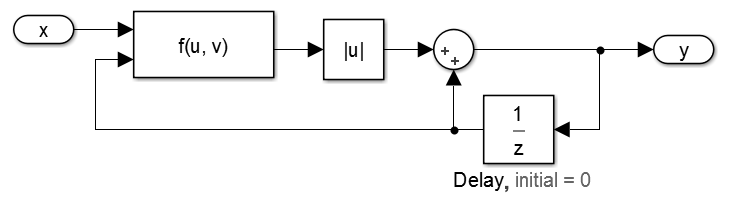
\includegraphics[width=\columnwidth]{figs/simulink.png}
%{\smaller
%\begin{verbatim}
%node filter(x : real) returns (a, b, y : real);
%let
%  a = f(x, 0.0 -> pre y);
%  b = if a >= 0.0 then a else -a;
%  y = b + (0.0 -> pre y);
%tel;
%\end{verbatim}
%}
%\vspace{-0.1in}
%\caption{Model with property $y \geq 0$, before IVC analysis}
%\label{fig:ex-before}
%\end{figure} 